%\documentclass{beamer}
\documentclass[serif]{beamer}
%--------------------------------------------------------------------------------------------------------------------------------------------
%----------------------------------------------------------PACKAGES---------------------------------------------------------------------
%--------------------------------------------------------------------------------------------------------------------------------------------
%\usepackage[T1]{fontenc}
%\usepackage{concmath}
\usepackage{beamerthemesplit}
\usepackage[utf8x]{inputenc}
\usepackage[italian, UKenglish]{babel}
%\usepackage [pdftex]{graphicx}
\usepackage [bf, small]{caption}
%\usepackage {caption}
\usepackage{mathtools}
\usepackage{tikz}
\usepackage{amsmath}
\usepackage{amsthm}
\usepackage{amssymb}
\usepackage{fancyhdr}
\usepackage{wrapfig}
\usepackage{subfigure}
\usepackage{newlfont}
\usepackage{hyperref}
\usepackage{verbatim}
\usepackage{leftidx}
\usepackage{mathabx}
%--------------------------------------------------------------------------------------------------------------------------------------------
%--------------------------------------------------NEW COMMANDS---------------------------------------------------------------------
%--------------------------------------------------------------------------------------------------------------------------------------------
%\usecolortheme[named=red]{structure}
%
\makeatletter
\newcommand\mathcircledred[1]{%
  \mathpalette\@mathcircledred{#1}%
}
\newcommand\@mathcircledred[2]{%
  \tikz[baseline=(math.base)] \node[draw,circle,inner sep=1pt, red] (math) {$\m@th#1#2$};%
}
\makeatother
%
\makeatletter
\newcommand\mathcircledgreen[1]{%
  \mathpalette\@mathcircledgreen{#1}%
}
\newcommand\@mathcircledgreen[2]{%
  \tikz[baseline=(math.base)] \node[draw,circle,inner sep=1pt, green] (math) {$\m@th#1#2$};%
}
\makeatother
%--------------------------------------------------------------------------------------------------------------------------------------------
%---------------------------------------------------------COMMANDS---------------------------------------------------------------------
%--------------------------------------------------------------------------------------------------------------------------------------------
%\theoremstyle{plain}
\theoremstyle{definition}
\newtheorem*{defin}{Definition}
\newtheorem*{obs}{Observation}
\newtheorem*{theor}{Theorem}
\newtheorem*{rec}{Recall}
\newtheorem*{prop}{Proposition}
\newtheorem*{no}{Notation}
\newtheorem*{pr}{Problem}
\newtheorem*{cor}{Corollary}
\newtheorem*{idea}{Idea}
%--------------------------------------------------------------------------------------------------------------------------------------------
%------------------------------------------------------------TITLE-------------------------------------------------------------------------
%--------------------------------------------------------------------------------------------------------------------------------------------
\title[Currents: an Interview] 
{Currents: an Interview}
%\subtitle
%{Include Only If Paper Has a Subtitle}
\author%[Giovanni Canarecci] % (optional, use only with lots of authors)
{Giovanni Canarecci}
% - Give the names in the same order as the appear in the paper.
% - Use the \inst{?} command only if the authors have different
%   affiliation.
\institute[University of Helsinki] % (optional, but mostly needed)
{
  Department of Mathematics and Statistics\\
  University of Helsinki
}
% - Use the \inst command only if there are several affiliations.
% - Keep it simple, no one is interested in your street address.
\date[18/05/2016] % (optional, should be abbreviation of conference name)
{18/05/2016}
% - Either use conference name or its abbreviation.
% - Not really informative to the audience, more for people (including
%   yourself) who are reading the slides online
% If you have a file called "university-logo-filename.xxx", where xxx is a graphic format that can be processed by latex or pdflatex, resp., then you can add a logo as follows:
\pgfdeclareimage[height=1cm]{university-logo}{HY_logo}
\logo{\pgfuseimage{university-logo}}
%
% Delete this, if you do not want the table of contents to pop up at
% the beginning of each subsection:
%\AtBeginSubsection[]
%{
%  \begin{frame}<beamer>{Content}
%    \tableofcontents[currentsection,currentsubsection]
%  \end{frame}
%}
%
% If you wish to uncover everything in a step-wise fashion, uncomment
% the following command: 
%\beamerdefaultoverlayspecification{<+->}
%--------------------------------------------------------------------------------------------------------------------------------------------
%----------------------------------------------------------DOCUMENT---------------------------------------------------------------------
%--------------------------------------------------------------------------------------------------------------------------------------------
\begin{document}


%\frame{\titlepage}
\begin{frame}
  \titlepage
\end{frame}

%------------------------------------------------------------------------------------------------------------------------------

%\section[CONTENTS]{}
%\begin{frame}{Contents}
%  \tableofcontents
  % You might wish to add the option [pausesections]
%\end{frame}

%------------------------------------------------------------------------------------------------------------------------------

\section{The Big Questions}
\subsection{Who do I study?}
\begin{frame}{Who do I study?}
I study \textbf{Currents} = linear functionals from the space of differential forms $\mathcal{D}^k(M)$ to the real line.
\begin{align*} 
S: \mathcal{D}^k(M) &\to \mathbb{R} \\
\varphi &\mapsto S(\varphi)
\end{align*}
where a differential form $\varphi$ is a map
$$
\varphi: \mathcal{T}(M) \to \mathbb{R}
$$
\end{frame}

%------------------------------------------------------------------------------------------------------------------------------

\subsection{How do I study them?}
\begin{frame}{How do I study them?}
We consider only those currents to whom we can associate a good set!
\begin{obs}
Any good\footnote{oriented $k-$dim rectifiable} set $\mathcircledgreen{S}$ can be seen as a current $\mathcircledred{S}$:
$$ \mathcircledred{S} : \varphi \in \mathcal{D}^{k}(M) \longrightarrow \int_{\mathcircledgreen{S}} \langle \overrightarrow{S}(x),\varphi \rangle \mu(x) d \mathcal{H}^k \in \mathbb{R}$$
And we call these currents "Rectifiable Currents".
\end{obs}
\end{frame}

%------------------------------------------------------------------------------------------------------------------------------

\subsection{Where do I study them?}
\begin{frame}{Where do I study them?}
In the Heisenberg Group:
$$
\mathbb{H}^1:= ( \mathbb{R}^3, * )
$$
that is $\mathbb{R}^3$ with a strange product:
$$
(x_1,y_1,t_1)*(x_2,y_2,t_2) = \left (x_1+x_2,y_1+y_2,t_1+t_2 \textcolor{red}{-2 (x_1y_2-x_2y_1)} \right ).
$$
\end{frame}

%------------------------------------------------------------------------------------------------------------------------------


\begin{frame}{Clear? ... maybe a picture would help!}
\begin{figure}
\centering
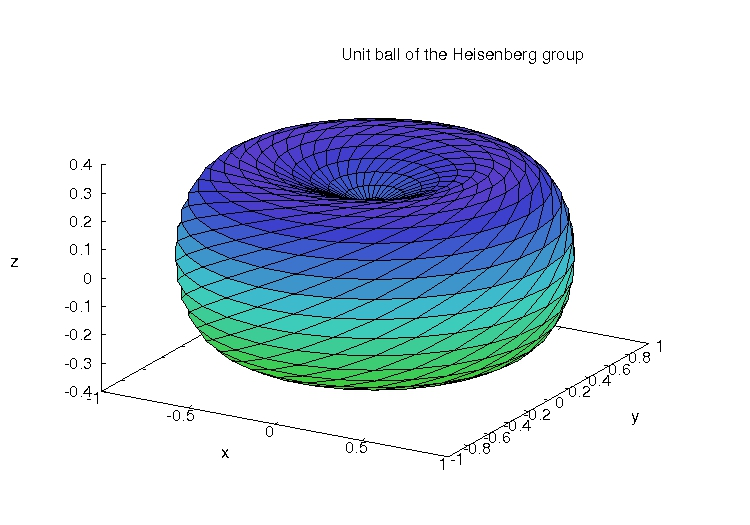
\includegraphics[width= 10 cm]{heisball.jpg}
\end{figure}
\end{frame}

%------------------------------------------------------------------------------------------------------------------------------

\subsection{What do I study with them?}
\begin{frame}{What do I study with them? The Plateau Problem!}
\begin{defin}[Plateau Problem]
Given a \textbf{boundary} with some kind of regularity, the Plateau Problem consists in finding the \textbf{minimal surface} that fits that boundary.
\end{defin}
\begin{figure}[!ht]
\centering
{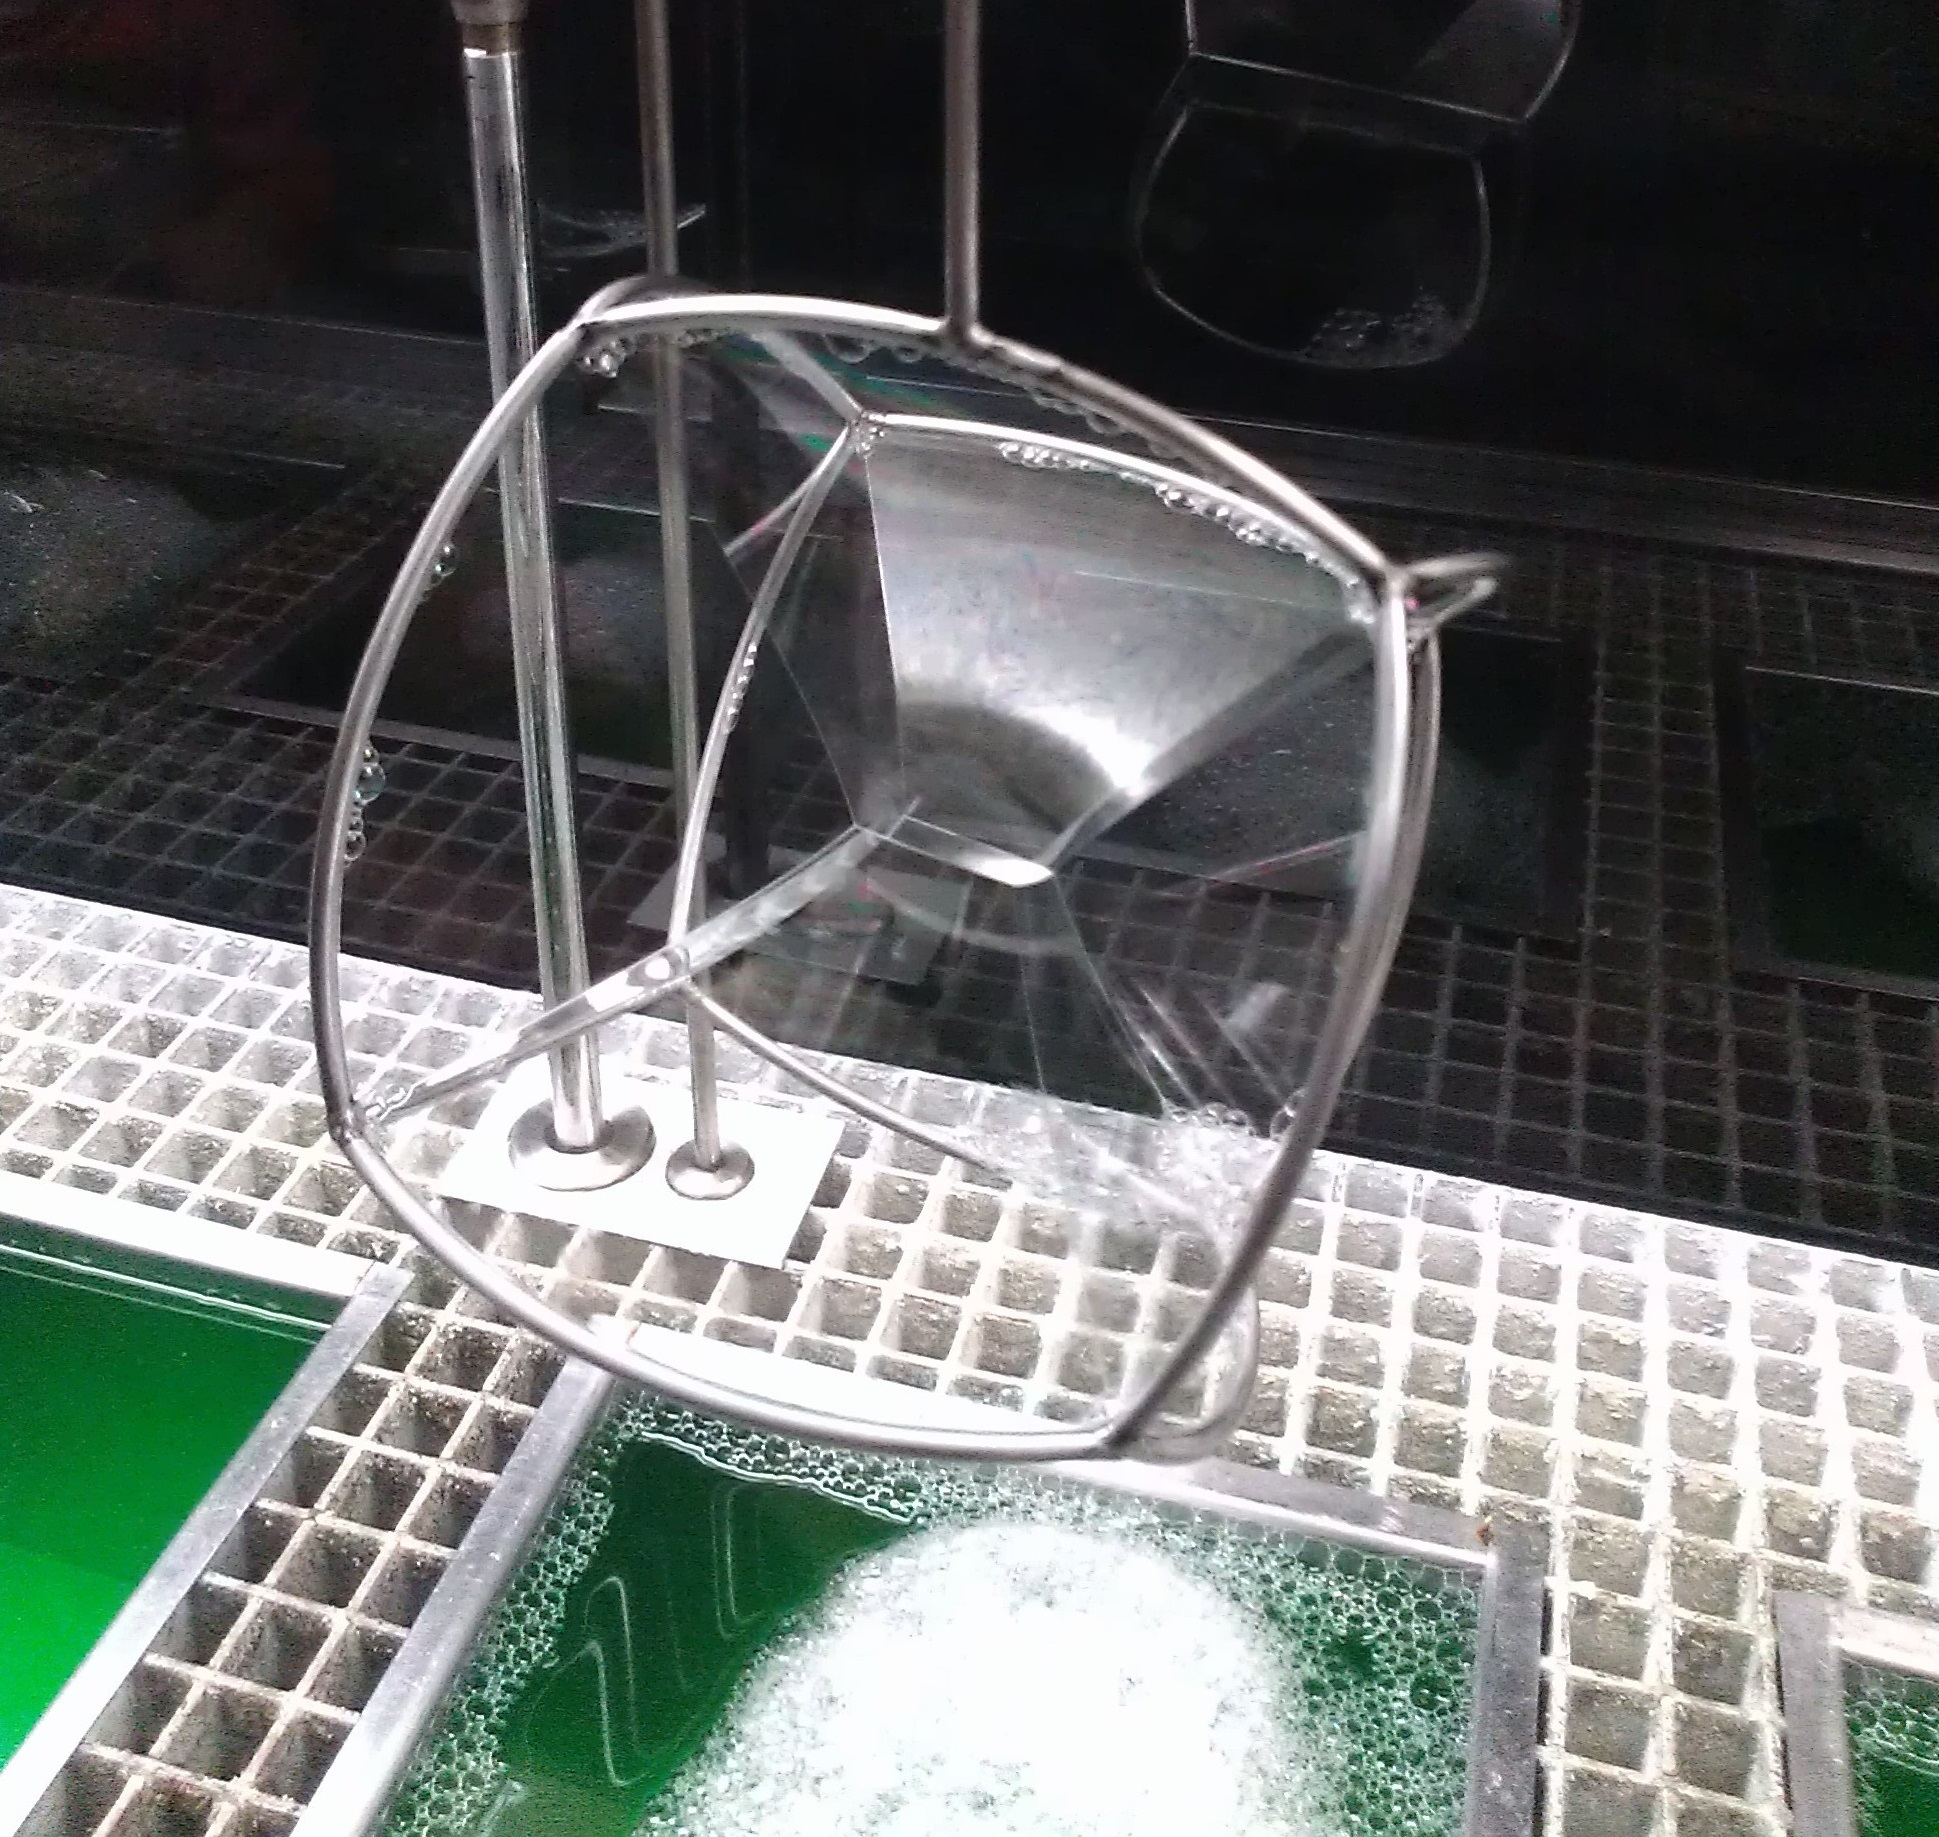
\includegraphics[width=4.5 cm]{Plateau_problem_01.jpg}}
{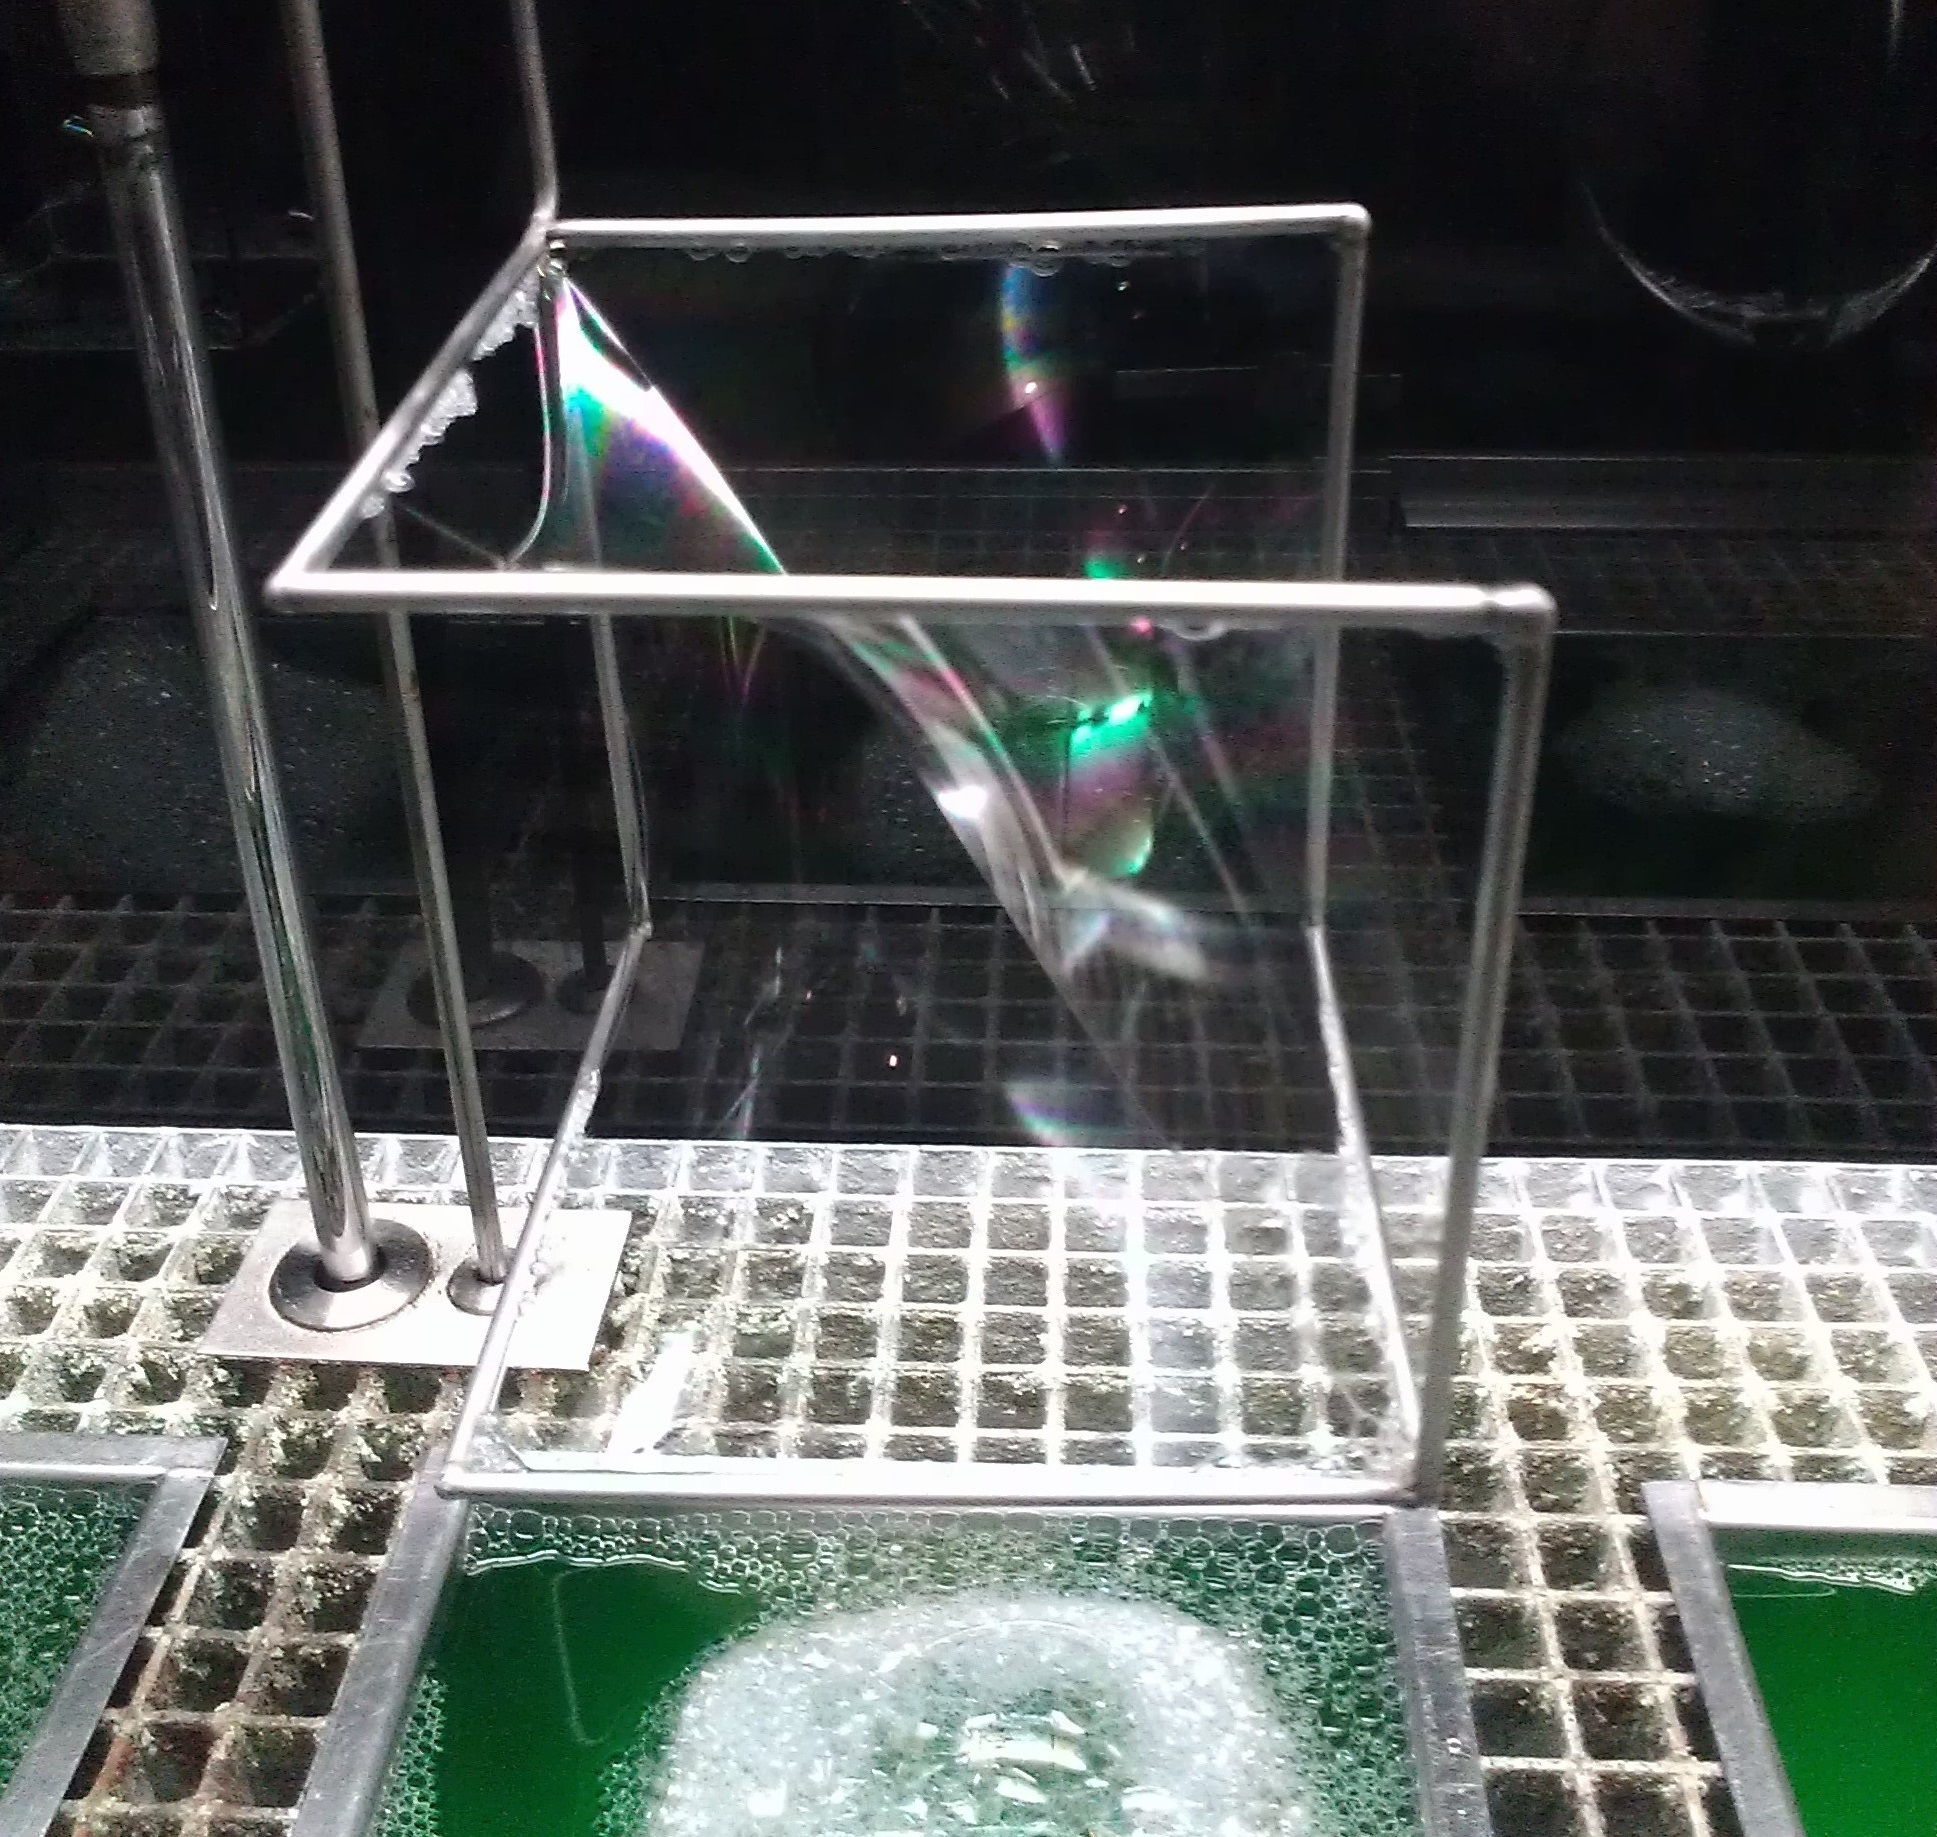
\includegraphics[width=4.5 cm]{Plateau_problem_02.jpg}}
\end{figure}
%\begin{figure}
%\centering
%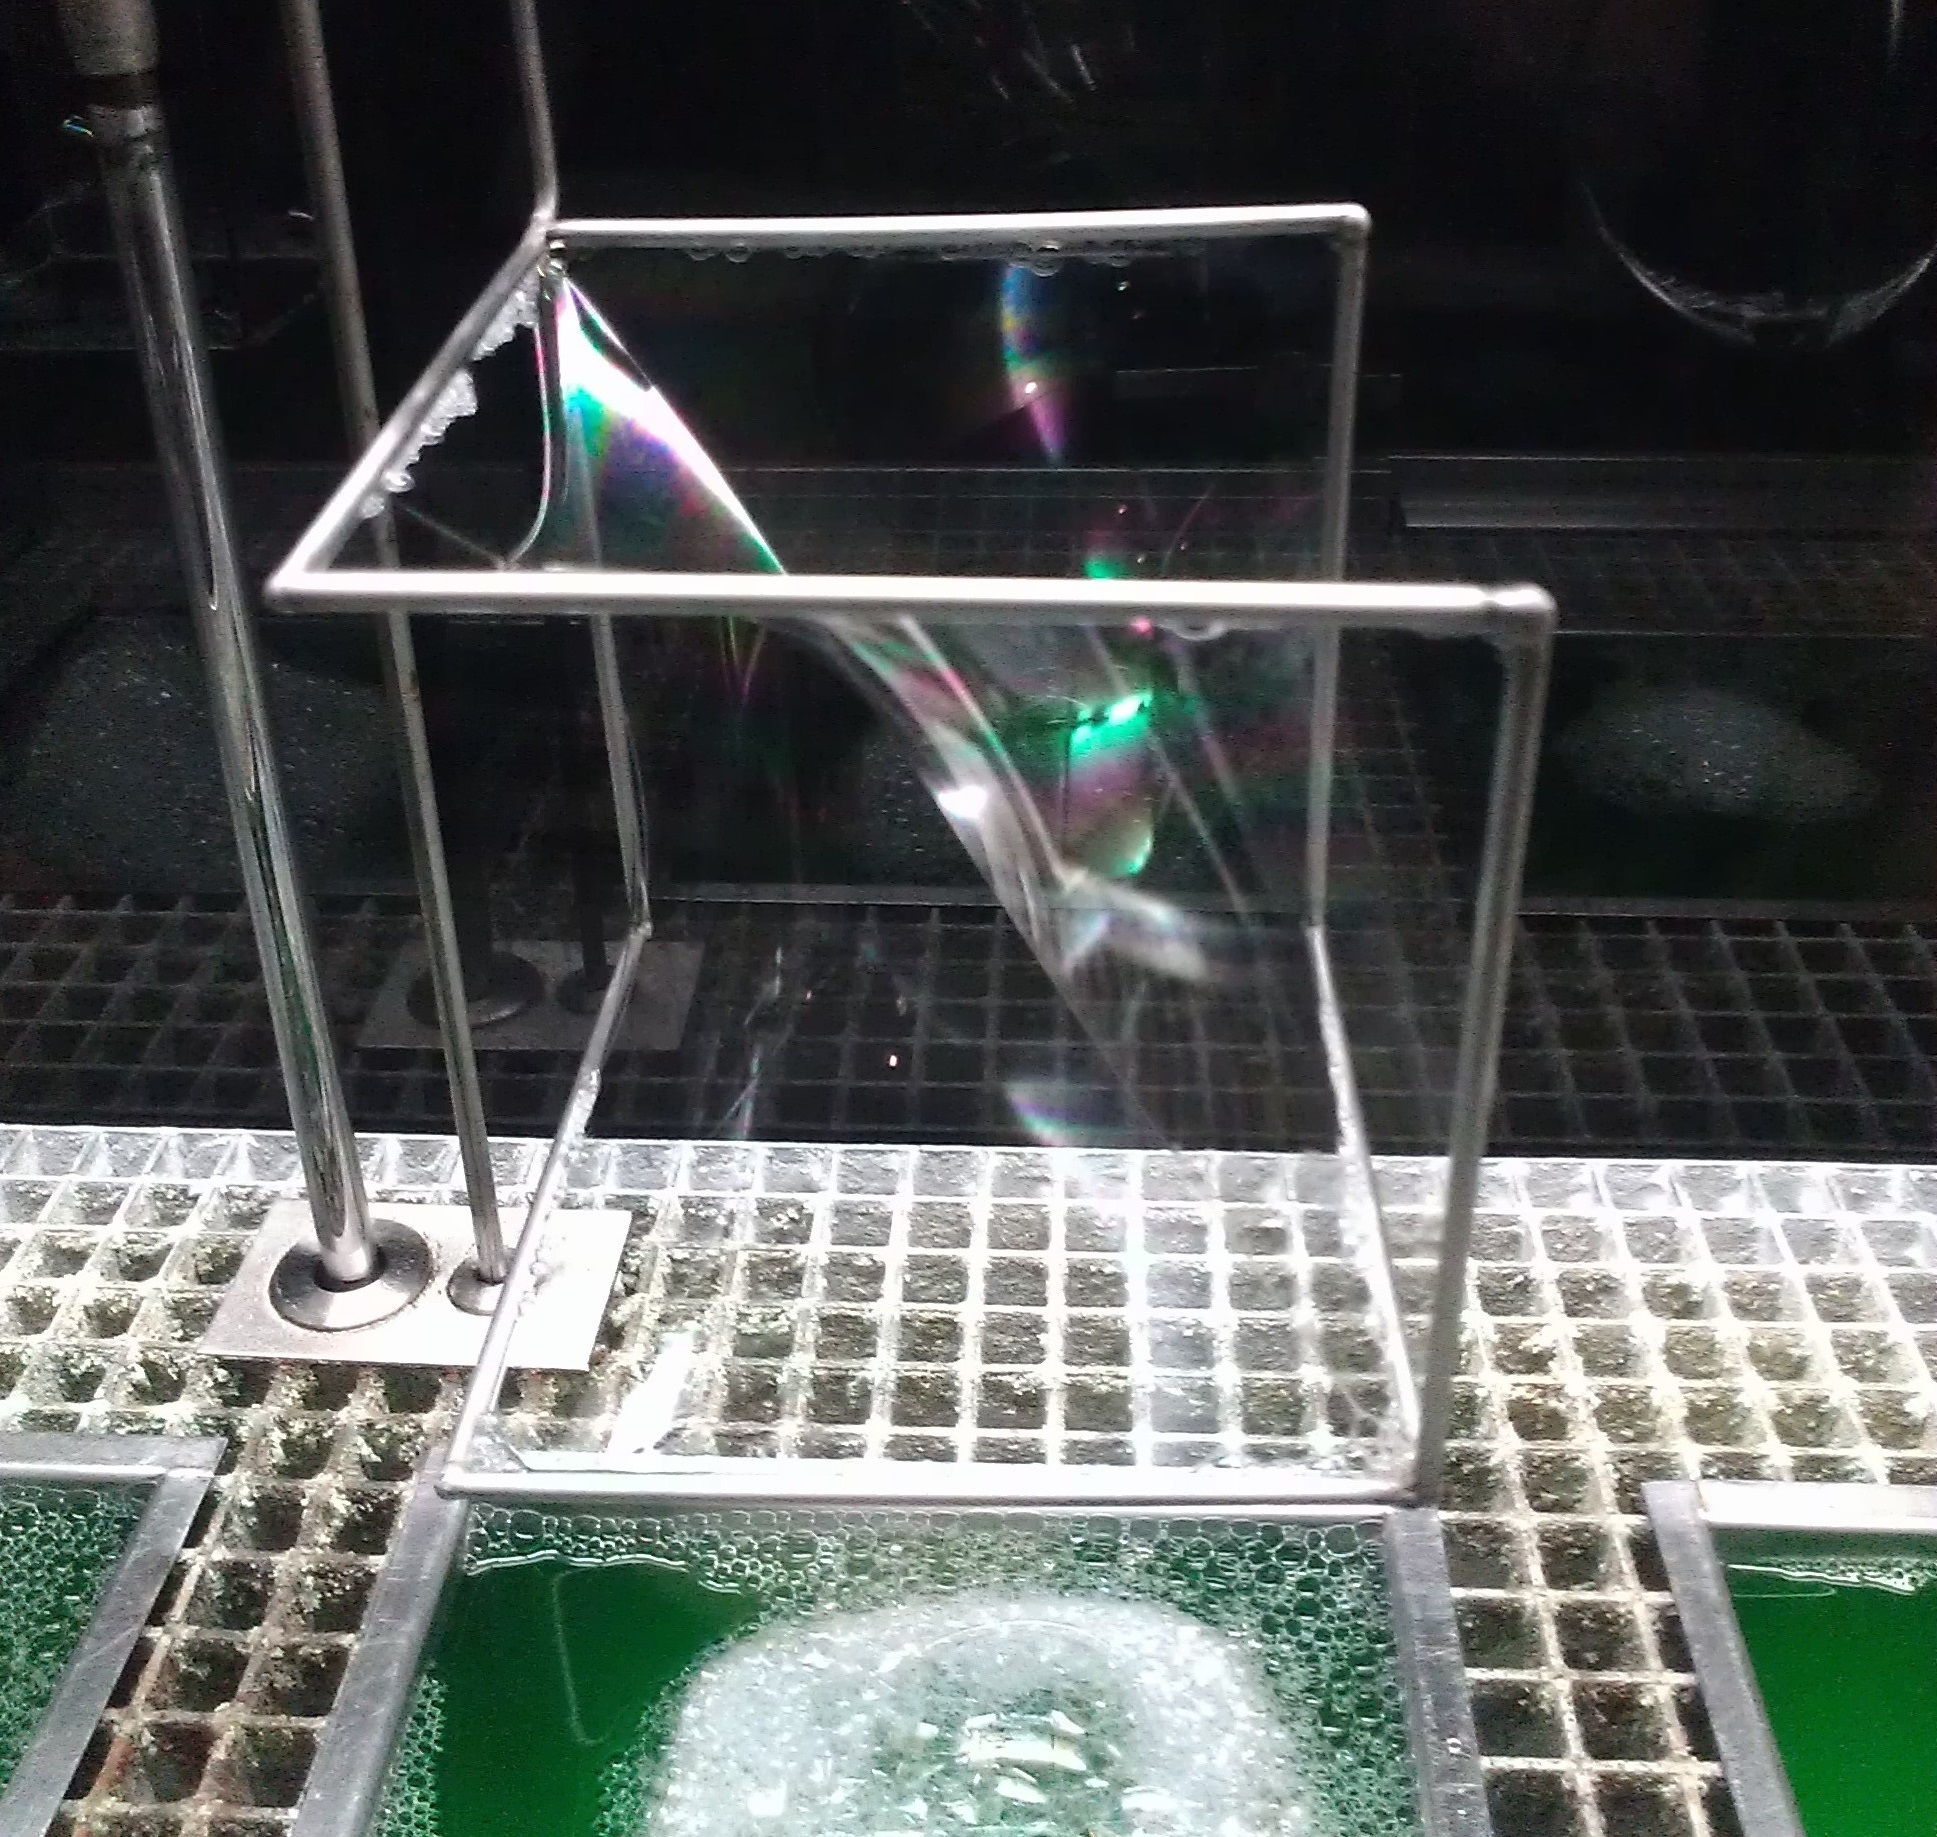
\includegraphics[width= 10 cm]{Plateau_problem_02.jpg}
%\end{figure}
\end{frame}

%------------------------------------------------------------------------------------------------------------------------------

\subsection{WHY?}
\begin{frame}{Why?}
A complete answer for this question is currently object of research.
\end{frame}

%------------------------------------------------------------------------------------------------------------------------------

\begin{frame}
\begin{center}
\huge{Kiitos paljon!}\\
\huge{Thank you!}\\
\huge{Grazie mille!}
\end{center}
\end{frame}

\end{document}%%%%%%%%%%%%
%------------------------------------------------------------------------------------------------------------------------------
%------------------------------------------------------------------------------------------------------------------------------
%------------------------------------------------------------------------------------------------------------------------------
%------------------------------------------------------------------------------------------------------------------------------
%------------------------------------------------------------------------------------------------------------------------------
